\documentclass[10pt,a4paper,oneside]{article}
\usepackage{cmap}
\usepackage[T2A]{fontenc}
\usepackage{float}
\usepackage{listings}
\usepackage{csquotes}
\usepackage[utf8]{inputenc}
\usepackage{amsmath}
\usepackage{amsfonts}
\usepackage{amssymb}
\usepackage[english, russian]{babel}%Подключаем русский язык.
\usepackage{graphicx}
\usepackage{geometry} % Меняем поля страницы.
\geometry{left=3cm} %Левое поле.
\geometry{right=2cm} %Правое поле.
\geometry{top=3cm} %Верхнее поле.
\geometry{bottom=2cm} %Нижнее поле.


%Начало документа
\begin{document}

%Создаём титульник.
\begin{titlepage}
\newpage
	%Название ВУЗа и институт.
	\begin{center}
		\Large Санкт-Петербургский Государственный Политехнический Университет\\
		Институт Компьютерных Наук и Технологий\\
	\end{center}
	%Кафедра.
	\begin{center}
		\large\textbf {Высшая школа интеллектуальных систем и суперкомпьютерных технологий}
	\end{center}
	
	%Пропуск места. 
	\vspace{5em}
	%!!!!!!!!!!!!!!!!!!!!!!!!!!!!!!!!!Название работы.
	\begin{center}
		\large{Отчёт по лабораторной работе №8 \\ на тему \\
		\textbf{Фильтрация и свертка} }
	\end{center}
	
	%Делаем пропуск и пишем студента и преподавателя.
	\vspace{25em}
	\begin{flushright}
		\textbf{Работу выполнил\\}Студент группы 3530901/80203 \\ Тарасенко Н.С.\\
		\textbf{Преподаватель\\}Богач Н.В. 
	\end{flushright}
	
	\vspace{\fill}%В самом низу
	\begin{center}
	Санкт-Петербург, 2021 год	
	\end{center}
\end{titlepage} %Закончили титульный лист.

\section{Настройка проекта}
Перед тем как выполнять задания необходимо настроить проект и сделать все необходимые импорты:

\begin{figure}[H]
        \centering
        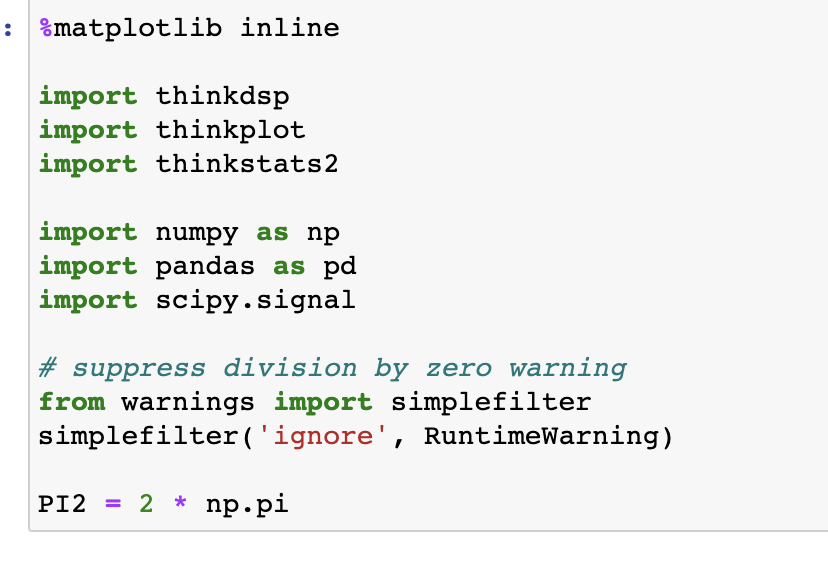
\includegraphics[width=0.75\textwidth]{0.png}
        \caption{2}
        \label{fig:first}
\end{figure}

\section{Упражнение номер №1}

Определить, что при увеличении ширины гауссова окна std не увеличивая число элементов в окне M

Если увеличивать ширину гауссова окна STD без увеличения количества элементов в окне M, это окно становится ближе к прямоугольному, более высокие частоты подавляются хуже, и следующие параметры проявляются боковым лепестком.

\section{Упражнение номер №2}

Определить, что происходит с преобразованием фурье, если меняется std

Рассмотрим Гауссовский пример:

\begin{figure}[H]
        \centering
        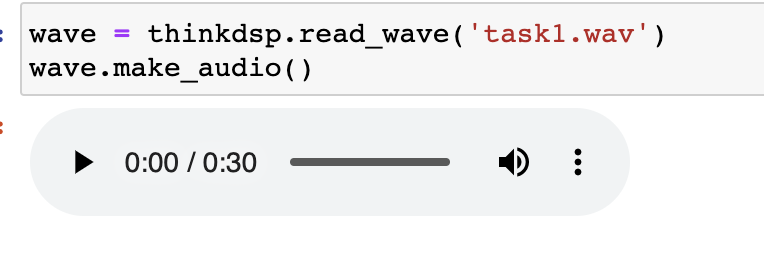
\includegraphics[width=0.75\textwidth]{1.png}
        \caption{2}
        \label{fig:first}
\end{figure}

Отобразим FFT:

\begin{figure}[H]
        \centering
        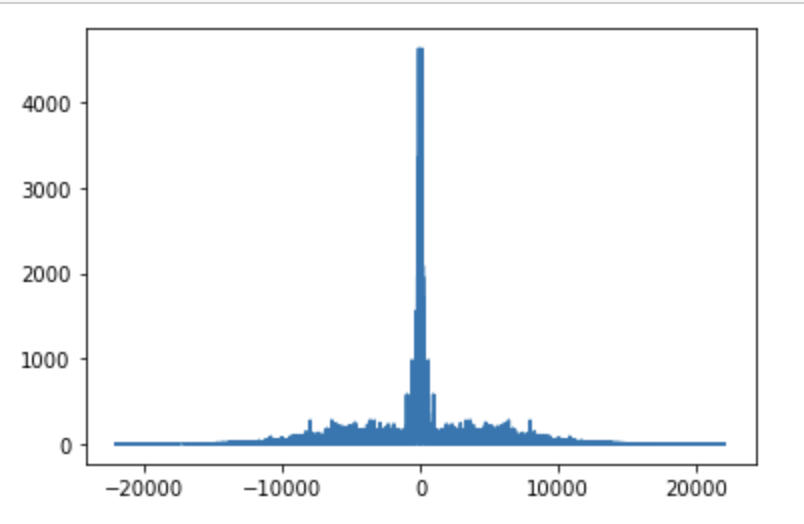
\includegraphics[width=0.75\textwidth]{2.png}
        \caption{2}
        \label{fig:first}
\end{figure}

В случае поворота отрицательных частот влево, то сможем более явно наблюдать Гауссовский пример:

\begin{figure}[H]
        \centering
        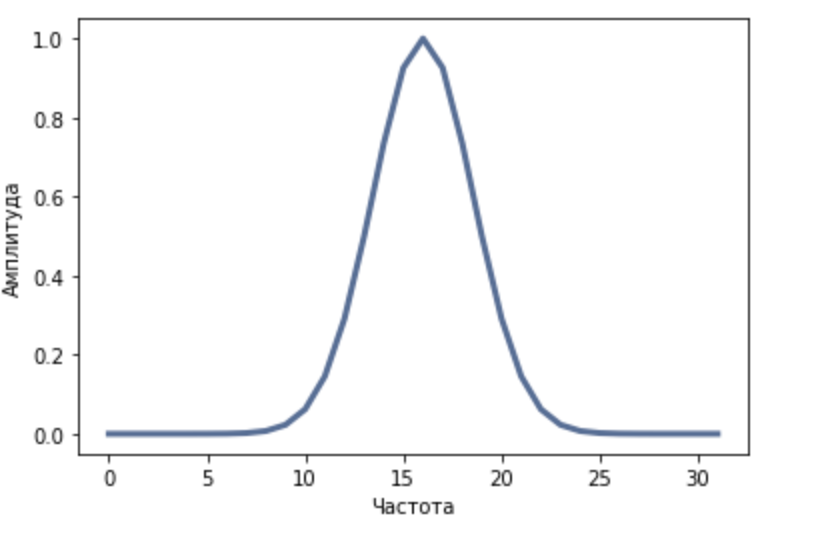
\includegraphics[width=0.75\textwidth]{3.png}
        \caption{2}
        \label{fig:first}
\end{figure}

С помощью данной функции мы можем увидеть окно Гаусса и его FFT:

\begin{figure}[H]
        \centering
        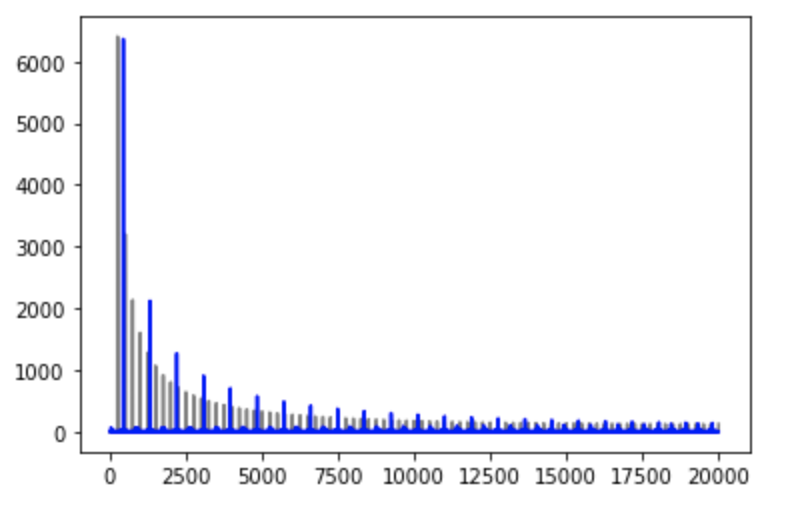
\includegraphics[width=0.75\textwidth]{4.png}
        \caption{2}
        \label{fig:first}
\end{figure}

Теперь мы можем проделать манипуляции, которые покажут, что произойдет при изменении std.

По мере увеличения std  Гауссовский становится шире, а его FFT сужается.

С точки зрения непрерывной математики, если

$f(x) = e^{-a x^2}$

который является гауссовским со средним 0 и стандартным отклонением $1/a$, его преобразование Фурье имеет вид

$F(k) = \sqrt{\frac{\pi}{a}} e^{-\pi^2 k^2/a}$

который является гауссовским со стандартным отклонением $a / \pi^2$. Таким образом, существует обратная зависимость между стандартными отклонениями $f$ и $F$.

\section{Упражнение номер №3}

Создать окно Хемминга тех размеров, что и Гаусса. Распечатать его ДПФ. Определить какое окно больше подходит для фильтрации НЧ.

Создадим волну в одну секунду с частотой дискретизации 44 кГц.

Затем создадим несколько окон. Выберем стандартное отклонение окна Гаусса, чтобы сделать его похожим на другие. Отобразим их:

\begin{figure}[H]
        \centering
        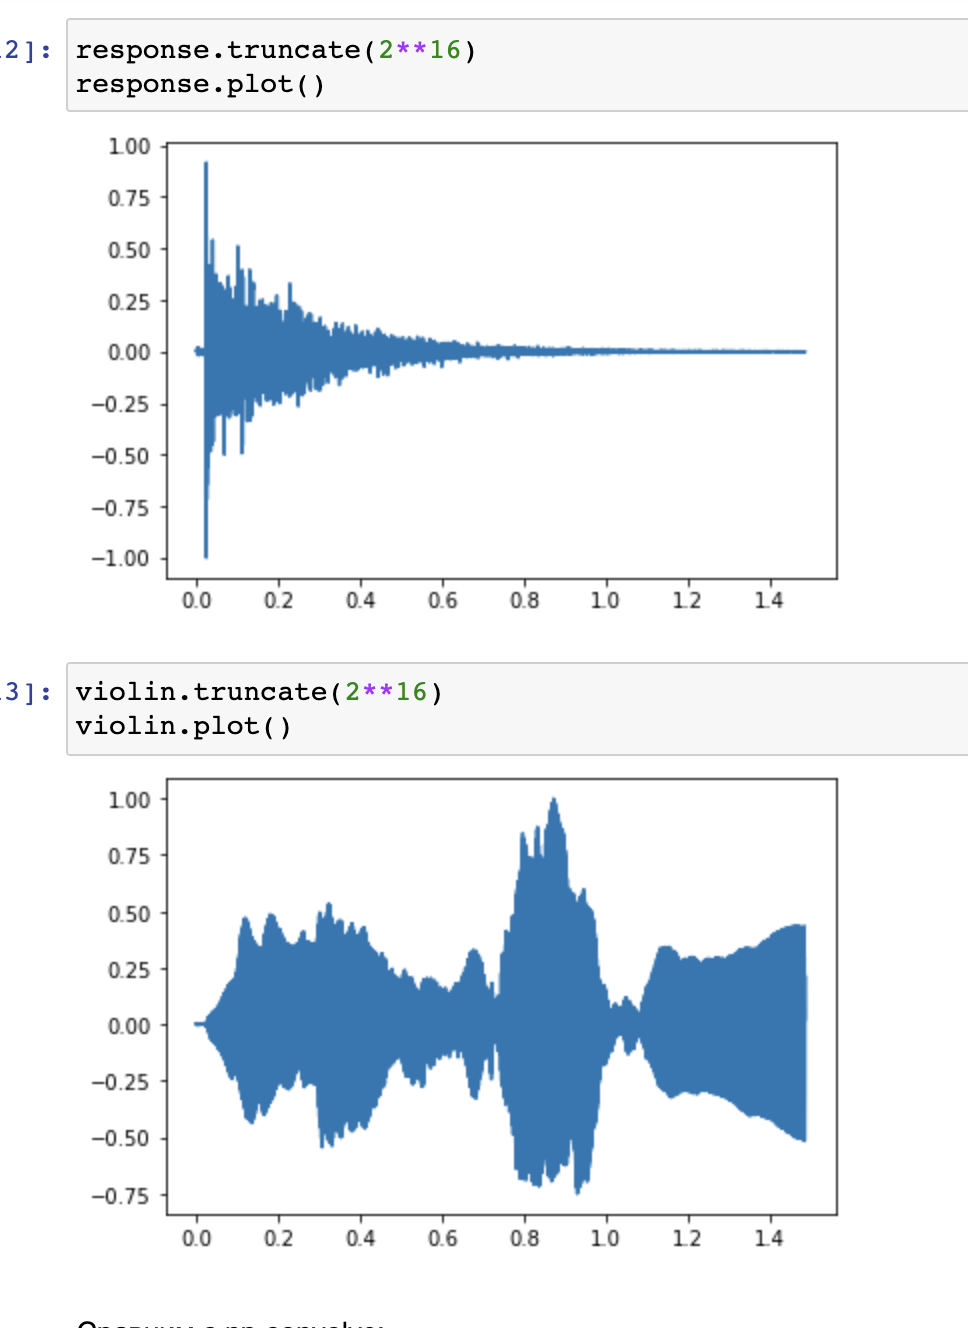
\includegraphics[width=0.75\textwidth]{5.png}
        \caption{2}
        \label{fig:first}
\end{figure}

Рассмотрим DFT:

\begin{figure}[H]
        \centering
        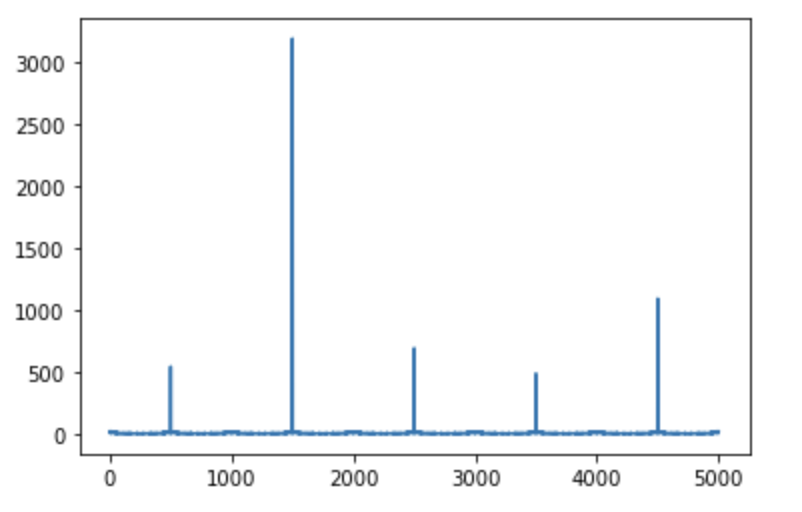
\includegraphics[width=0.75\textwidth]{6.png}
        \caption{2}
        \label{fig:first}
\end{figure}

Стоит отметить, что Гауссово падает быстрее всех, Блэкман - самым медленным, а у Ханнинга самые заметные боковые лепестки

В логарифмической шкале мы видим, что сначала значения Хэмминга и Хеннинга падают быстрее, чем два других. И окна Хэмминга и Гаусса, кажется, имеют самые стойкие боковые лепестки. Окно Ханнинга может иметь наилучшее сочетание быстрого падения и минимальных боковых лепестков.

\begin{figure}[H]
        \centering
        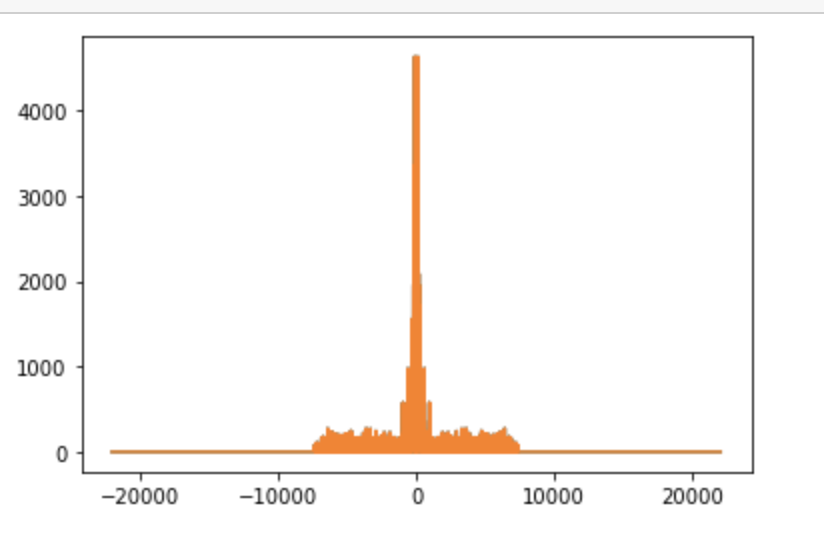
\includegraphics[width=0.75\textwidth]{7.png}
        \caption{2}
        \label{fig:first}
\end{figure}


\end{document}